% Chapter Template

\chapter{Literature review and Overall Description} % Main chapter title

\label{Chapter2} % Change X to a consecutive number; for referencing this chapter elsewhere, use \ref{ChapterX}

\lhead{Chapter 2. \emph{Literature review and Overall Description}} % Change X to a consecutive number; this is for the header on each page - perhaps a shortened title

%----------------------------------------------------------------------------------------
%	SECTION 1
%----------------------------------------------------------------------------------------

\section{LITERATURE REVIEW}\label{sec:2.1}

\textbf THE EYE STICK – WALKING STICK THAT SEES\\
Methodology - The Eye Stick is fitted with a sensor lens towards the bottom part, from where it picks up location bearings, like is the person nearing a staircase, or is he near the traffic lights. It then sends feedback to the blind commuter via sonic vibrations, communicating the scenario, so that the person can be aware of his surroundings and take his next step with confidence.
Result - The blind person can recognize where they are through the Eye Stick. They can avoid dangerous things as well as locate their destination. The eye stick can also recognize traffic light signals, stair steps, and the subway station. Show in Figure \ref{fig:2_1} and \ref{fig:2_2}\\

\begin{figure}[t]
	\centering
	\begin{subfigure}[b]{0.4\textwidth}
		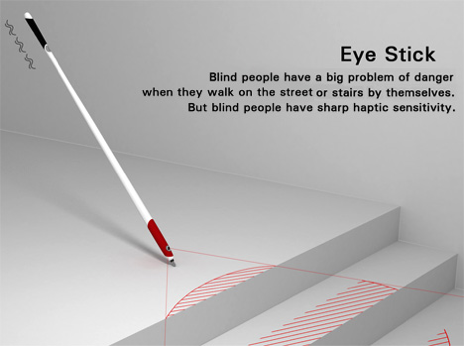
\includegraphics[width=\textwidth]{2_1.png}
		\caption{}
		\label{fig:2_1}
	\end{subfigure}
	\begin{subfigure}[b]{0.39\textwidth}
		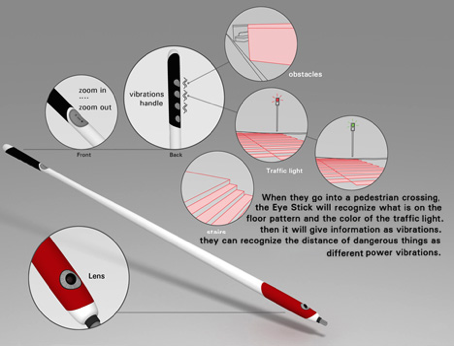
\includegraphics[width=\textwidth]{2_2.png}
		\caption{}
		\label{fig:2_2}
	\end{subfigure}
	\caption{(a) and (b) The eye stick - Walking stick that sees}
\end{figure}

\textbf PLASTIC FANTASTIC BRAIN\\
Methodology – allow blind to see image from vibrations simulated from user’s tongue. The equipment component are camera and tiny electric pinprict. When the blind wear a camera on their head. The camera will capture the object in front of them. When taking a tiny electric pinprict in user’s mouth, it will draw a picture of an object directly on the surface of user’s tongue. This information is represented in a form of a picture. Which is later translated by visual cortex of user’s brain.\\
Result – Blind people use their tongue to locate an object and identify its shape. Show in figure 
\ref{fig:2_3} , \ref{fig:2_4} and \ref{fig:2_5}

\begin{figure}[t]
	\centering
	\begin{subfigure}[b]{0.4\textwidth}
		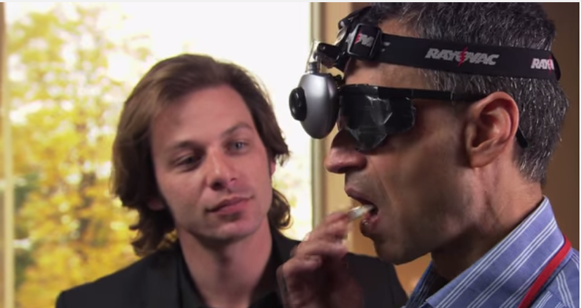
\includegraphics[width=\textwidth]{2_3.png}
		\caption{}
		\label{fig:2_3}
	\end{subfigure}\\
	\begin{subfigure}[b]{0.39\textwidth}
		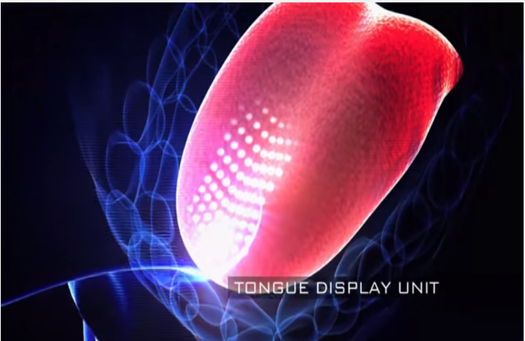
\includegraphics[width=\textwidth]{2_4.png}
		\caption{}
		\label{fig:2_4}
	\end{subfigure}\\
	\begin{subfigure}[b]{0.39\textwidth}
		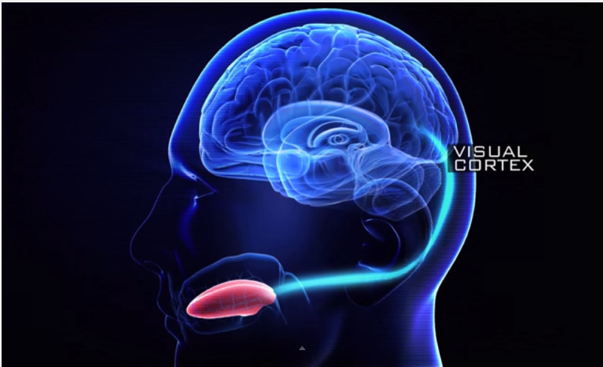
\includegraphics[width=\textwidth]{2_5.png}
		\caption{}
		\label{fig:2_5}
	\end{subfigure}\\
	\caption{(a) , (b) and (c) Plastic Fantastic Brain}
\end{figure}


\section{Overall Description}
Obstacle Avoidance System is an embedded-system intended to assist a person with severe vision disabilities. Working as a cane complementary, the system is able to detect distance further than a cane can reach
The system uses a proximity sensor attached at the belt. The system detects the closest object within its proximity and sends it to vibration sensor signaling an incoming obstacles. Moreover, the system can also detect possibility of human presence. It help ensures user that an object they are currently looking may likely be human. They can act accordingly\\

\textbf USER CLASSES AND CHARACTERISTICS\\
This product focus mainly on person with severe vision disabilities who has visual field less than 10 degrees. The product also focus on a person with complete blindness, unable to sense light source from an environment as well.

\textbf OPERATING ENVIRONMENT\\

